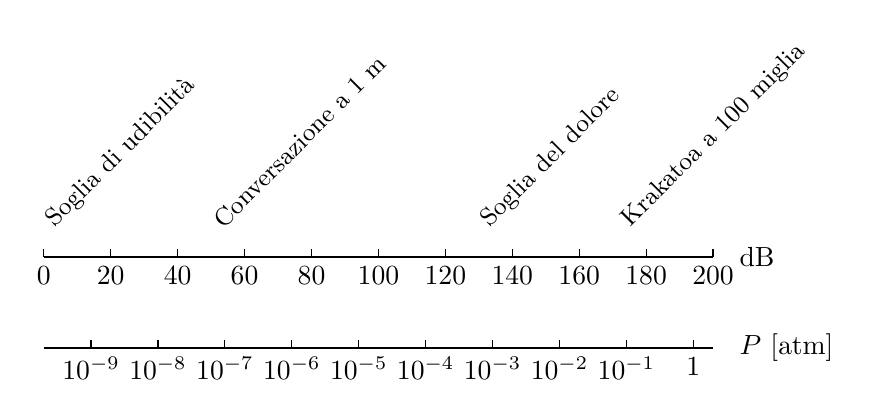
\begin{tikzpicture}[declare function={dbdist(\x)=\xscale*20*(10+\x-log10(1.97));}]%
  \node at (0, 0) {};
  \pgfmathsetmacro{\xscale}{0.0425}

  \pgfmathsetmacro{\y}{0.25}
  {\small
    \node[anchor=west,rotate=45] at (\xscale*0, \y) {Soglia di udibilit\`a};
    \node[anchor=west,rotate=45] at (\xscale*50, \y) {Conversazione a $1$~m};
    \node[anchor=west,rotate=45] at (\xscale*130, \y) {Soglia del dolore};
    \node[anchor=west,rotate=45] at (\xscale*172, \y) {Krakatoa a~100 miglia};
  }

  \pgfmathsetmacro{\y}{-0.1}
  \draw[thick] (0,\y) -- (\xscale*200,\y);
  \node[anchor=west] at (\xscale*205,\y) {dB};
  \foreach \x in {0.,20,...,200}
  \draw (\x*\xscale,\y+0.1) -- (\x*\xscale,\y) node[anchor=north]
        {$\pgfmathprintnumber{\x}$};

  \pgfmathsetmacro{\y}{-1.25}
  \draw[thick] (0,\y) -- (\xscale*200,\y);
  \node[anchor=west] at (\xscale*205,\y) {$P$~[atm]};
  \draw ({dbdist(-9)},\y+0.1) -- ({dbdist(-9)},\y) node[anchor=north] {$10^{-9}$};
  \draw ({dbdist(-8)},\y+0.1) -- ({dbdist(-8)},\y) node[anchor=north] {$10^{-8}$};
  \draw ({dbdist(-7)},\y+0.1) -- ({dbdist(-7)},\y) node[anchor=north] {$10^{-7}$};
  \draw ({dbdist(-6)},\y+0.1) -- ({dbdist(-6)},\y) node[anchor=north] {$10^{-6}$};
  \draw ({dbdist(-5)},\y+0.1) -- ({dbdist(-5)},\y) node[anchor=north] {$10^{-5}$};
  \draw ({dbdist(-4)},\y+0.1) -- ({dbdist(-4)},\y) node[anchor=north] {$10^{-4}$};
  \draw ({dbdist(-3)},\y+0.1) -- ({dbdist(-3)},\y) node[anchor=north] {$10^{-3}$};
  \draw ({dbdist(-2)},\y+0.1) -- ({dbdist(-2)},\y) node[anchor=north] {$10^{-2}$};
  \draw ({dbdist(-1)},\y+0.1) -- ({dbdist(-1)},\y) node[anchor=north] {$10^{-1}$};
  \draw ({dbdist(0)},\y+0.1) -- ({dbdist(0)},\y) node[anchor=north] {$1$};
\end{tikzpicture}
